\chapter{یادگیری ماشین}
در سال 1959، آرتور ساموئل اصطلاح یادگیری ماشین را به عنوان زمینه‌ای که به کامپیوتر توانایی یادگیری بدون برنامه‌ریزی صریح را می‌دهد ابداع کرد،. چهار دسته گسترده از مسائل وجود دارد که می‌توان از یادگیری ماشین در آنها استفاده‌کرد:
\begin{enumerate}
    \item خوشه‌ بندی\LTRfootnote{\lr{Clustering}}:
    گروه بندی داده‌های مشابه باهم با افزایش فاصله بین گروه‌ها 
    \item طبقه ‌بندی\LTRfootnote{\lr{Classification}}: نگاشت مجموعه‌ای از داده‌های جدید به مجموعه‌ای با مقادیر گسسته 
    \item رگرسیون\LTRfootnote{\lr{Regression}}: نگاشت مجموعه‌ای از داده‌های جدید به مجموعه‌ای با مقادیر پیوسته
    \item استخراج قاعده\LTRfootnote{\lr{Rule Extraction}}: شناسایی روابط آماری در داده‌ها 
\end{enumerate}

روشی کلی برای ساختن راه حل‌های مبتنی بر یادگیری ماشین وجود دارد \cref{fig.1}. که در ادامه به بررسی مختصر هرکدام از اجزا می‌پردازیم.

\begin{figure}[!h]
\centering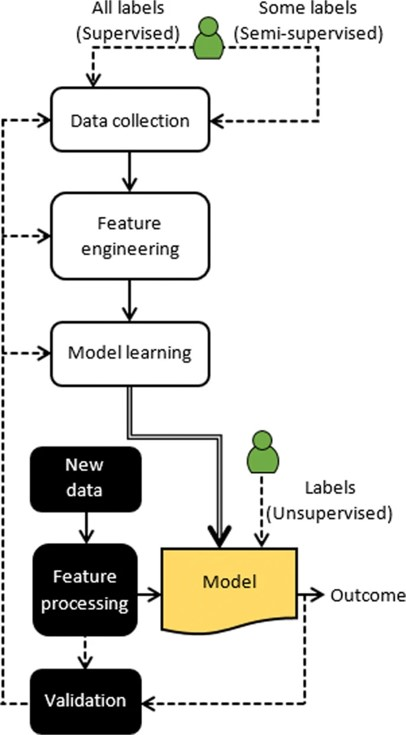
\includegraphics[scale=.8]{./figures/Solution}
\caption{اجزاء سازنده‌ی راه حل‌های مبتنی بر یادگیری ماشین}\label{fig.1}
\end{figure}

\newpage

\section{الگوهای یادگیری}

در یادگیری ماشین چهار الگوی یادگیری وجود دارد، این الگوها بر مراحل بعدی تأثیر می‌گذارند. هدف کلی این است که با توجه به برخی از مجموعه‌های داده نتیجه بگیریم. این الگوها برپایه‌ی دو روش فکری مولد  \LTRfootnote{\lr{Generative}}  و متمایزکننده \LTRfootnote{\lr{Discriminative}} هستند که ریشه در قانون بیز  \LTRfootnote{\lr{Bayes’ Theorem}} دارند:

\begin{equation}
    P(A|B) = \frac{P(B|A)*P(A)}{P(B)}
\end{equation}

%$$
%P(A|B) = \frac{P(B|A)*P(A)}{P(B)}
%$$
این چهار الگوی یادگیری عبارتند از:
\begin{itemize}
\item تحت نظارت\LTRfootnote{\lr{Supervised Learning}}: در حل مسائل طبقه‌بندی و رگرسیون کاربرد دارد و از مجموعه داده‌های برچسب‌دار برای مدل کردن استفاده می‌کنند.
\item نیمه نظارت\LTRfootnote{\lr{Semi-supervised Learning}}: اگر برچسب‌ها ناقص باشند از یادگیری نیمه نظارتی استفاده می‌شود.
\item بدون نظارت\LTRfootnote{\lr{Unsupervised Learning}}: اگر داده‌ها بی‌برچسب باشند از یادگیری بدون نظارت استفاده خواهد شد. از این روش بیشتر در مسائل خوشه بندی استفاده می‌شود.
\item تقویتی\LTRfootnote{\lr{Reinforcement Learning(RL)}}: یک فرایند تکراری مبتنی بر عامل است. عامل در محیط به کاوش می‌پردازد و درنهایت آن را بر اساس اعمالش تشویق و یا جریمه می‌کند. درواقع مجموعه داده‌ها شامل همین تشویق و جریمه‌ها می‌باشند. همچنین با دریافت بازخورد از محیط، کاوش‌های بعدی را تعیین می‌شود.
\end{itemize}



\newpage


\section{جمع‌آوری داده}

تکنیک‌های یادگیری ماشین برای ساخت یک مدل موثر یادگیری ماشین برای یک مشکل خاص، نیاز به داده دارند. جمع آوری داده‌ها یک مرحله مهم است، زیرا داده‌ها نه تنها از یک مسئله به مسئله دیگر بلکه در دوره‌های زمانی نیز باهم متفاوت هستند. به طور کلی جمع آوری داده در دو فاز انجام میشود:
\begin{itemize}
\item آفلاین: این امکان را به ما می‌دهد تا داده‌های مربوط به گذشته برای آموزش و تست مدل به کار روند.
\item آنلاین: این امکان را به ما می‌دهد تا داده‌های شبکه در زمان حال برای بازخورد و ورودی برای آموزش مجدد به کار روند.
\end{itemize}

یک منبع برای جمع آوری داده در هر دوفاز استفاده از ابزارهای نظارتی و اندازه گیری، در سطح شبکه است که میتواند به صورت‌های زیر باشد:

\begin{itemize}
\item نظارت فعال: ترافیک اندازه گیری را تزریق می‌کند، مانند بسته‌های پروب \LTRfootnote{\lr{Probe}} در شبکه و داده‌های مربوطه را از این ترافیک جمع آوری می‌کند.
\item نظارت غیرفعال: با مشاهده میزان واقعی ترافیک شبکه، داده‌ها را جمع آوری می‌کند.
\end{itemize}

نظارت فعال به دلیل مصرف پهنای باند از ترافیک تزریقی، هزینه اضافی را به دنبال دارد. در حالیکه، نظارت غیرفعال با هزینه دستگاه‌های اضافی که ترافیک شبکه را برای جمع آوری اطلاعات مربوطه تجزیه و تحلیل می‌کنند، این سربار را از بین می‌برد\cite{ boutaba2018comprehensive}.
\\
پس از جمع آوری داده‌ها، آنها به مجموعه‌های آموزش، اعتبار سنجی و آزمون تجزیه می‌شوند. مجموعه آموزش برای یافتن پارامترهای ایده آل، مجموعه اعتبار سنجی برای انتخاب معماری مناسب و مجموعه آزمون برای ارزیابی عملکرد بی‌طرفانه مدل انتخاب شده استفاده می‌شود. اینکه چه درصدی از داده‌ها را به کدام مجموعه اختصاص دهیم باید با توجه به کلاس‌های مورد علاقه صورت گیرد.
\newpage

\section{مهندسی ویژگی}



داده‌های خام جمع آوری شده ممکن است اضافی یا ناقص باشند. قبل از استفاده از داده‌ها برای یادگیری، باید مرحله قبل از پردازش را طی کرد. مرحله مهم دیگر قبل از یادگیری، یا آموزش یک مدل، استخراج ویژگی است.


مهندسی ویژگی یک جنبه حیاتی در یادگیری ماشین است که شامل انتخاب و استخراج ویژگی است. برای کاهش ابعاد در داده‌های حجیم و شناسایی ویژگی‌های متمایز که سربار محاسباتی را کاهش می‌دهد استفاده می‌شود. استخراج ویژگی‌ها معمولاً یک فرآیند محاسباتی فشرده است که با استفاده از تکنیک‌هایی مانند آنتروپی و تبدیل فوریه از ویژگی‌های موجود می‌توان ویژگی‌های جدیدی را به دست آورد\cite{ boutaba2018comprehensive}.


\section{ایجاد حقیقت عینی}


ایجاد حقیقت عینی درواقع دادن توصیف رسمی (به عنوان مثال برچسب) به کلاس‌های مورد علاقه است. حقیقت عینی دقت مدل‌های یادگیری ماشین را به همراه دارد. همچنین وابستگی متقابل بین داده‌های آموزشی یک کلاس مورد علاقه به کلاس دیگر وجود دارد که بر عملکرد مدل تأثیر می گذارد. عدم تعادل در تعداد داده‌های آموزش در بین کلاس ها، فرضیاتی را که بسیاری از تکنیک‌های یادگیری ماشین دارند، نقض میکند. بنابر این با استفاده از انواع روش‌های نمونه برداری باید تعادل را برقرار کرد\cite{ boutaba2018comprehensive}.



\section{شاخص‌های عملکرد و اعتبارسنجی مدل}

هنگامی که یک مدل یادگیری ماشین ساخته شد و حقیقت عینی مشخص شد، ارزیابی عملکرد مدل یادگیری ماشین که نتایج را توصیف، پیش بینی یا ارزیابی می‌کند، بسیار مهم است. همچنین، باید توجه کنیم که هیچ راهی برای تشخیص الگوریتم یادگیری به عنوان بهترین الگوریتم وجود ندارد و مقایسه میزان خطا در طیف وسیعی از برنامه‌ها عادلانه نیست. از معیارهای عملکرد می‌توان برای اندازه گیری جنبه‌های مختلف مدل مانند قابلیت اطمینان، استحکام، دقت و پیچیدگی استفاده کرد.

%\section{تکامل روش‌های یادگیری ماشین}

\newpage

\section{خلاصه}


در این فصل، روشي كلي براي ساختن راه حل هاي مبتني بر يادگيري ماشين را ارائه دادیم. در ابتدا، انواع الگوهای یادگیری تحت نظارت، نیمه نظارت، بدون نظارت و تقویتی را دیدیم. سپس مرحله جمع آوری داده ها وجود دارد که به صورت آفلاین و آنلاین انجام می‌شود. سپس به سراغ استخراج ویژگی‌ها رفتیم که برای جلوگیری از سربار محاسباتی مرحله‌ای مهم است. بعد از آن ایجاد حقیقت عینی را دیدیم که می‌بایست به نحوی انجام بشود که تعادل در تعداد داده‌های آموزش برقرار شود. و در مرحله آخر می‌بایست مدل تولید شده را مورد اعتبارسنجی و ارزیابی قرار داد.

